\chapter{Evaluation}
\label{chap:Evaluation}

\section{Section1}
\paragraph{paragraph1}
\subsection{Features}
Dans une tâche d'object detection, nous utilisons le score IoU qui signifie Intersection over Union.
C'est un score qui compare les bounding boxes prédites par le modèle avec les bounding boxes réels (ground-truth).
\begin{figure}[tbh!]
    \centering
    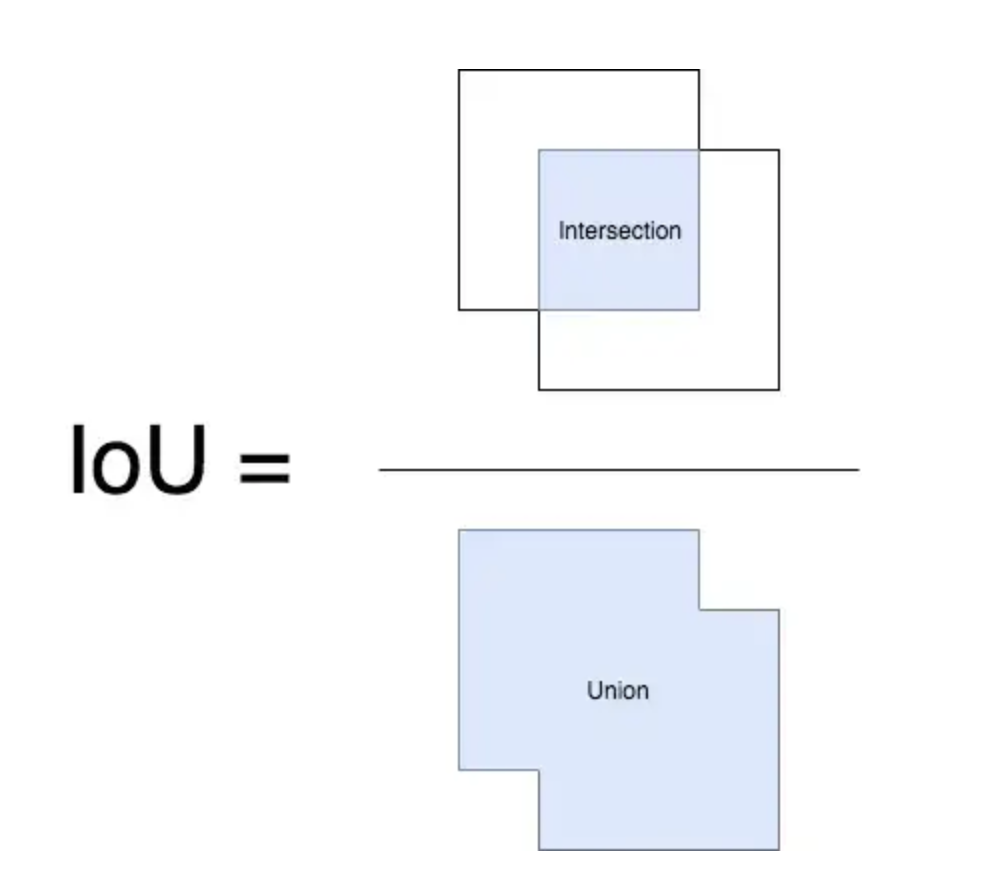
\includegraphics[width=\textwidth]{images/iou.png}
    \caption{Intersection over Union}
    \label{fig:iou}
\end{figure}
Une tâche d'object detection comprend deux sous-problèmes: la classification et la localisation.
Ainsi nous avons plusieurs métriques pour analyser la performance d'un modèle. IoU se concentre sur l
a localisation des bounding box prédites tandis que la métrique mAP (mean Average Precision) 
se concentre sur la classification.

% -- Vic : 

\section{Résultats des modèles fonctionnels choisis}

Après avoir testé plusieurs approches comme mentionnées dans le chapitre \autoref{chap:Modeles}

modele
mAP ou AP (?)
IoU50
IoU95

--> modèle final choisi 

Entraînement : 

Validation (résultats) important de dire que images sont similaires à celles deja vues blabla

Prédiction : ajout d'un treshold qui prend slmt prédictions avec une proba de + de blabla
